\documentclass[a4paper,11pt,eval]{nsi} 
\usepackage{fontawesome5}

%\pagestyle{empty}


\newcounter{exoNum}
\setcounter{exoNum}{0}
%
\newcommand{\exo}[1]
{
	\addtocounter{exoNum}{1}
	{\titlefont\color{UGLiBlue}\Large Exercice\ \theexoNum\ \normalsize{#1}}\smallskip	
}



\begin{document}



%\textcolor{UGLiBlue}{Mercredi 05/02/2025}\\
\classe{\terminale Comp}
\titre{Préparation de l'évaluation-bilan 4}
\maketitle
\begin{center}
	Calculatrice autorisée. Toutes les réponses doivent être justifiées.
\end{center}

\vspace*{1cm}


\dleft{11.5cm}{
    \exo{}\\
    Dans une kermesse, on fait tourner la roue de loterie équilibrée ci-contre où tous les secteurs ont le même angle.\\
    Le joueur gagne le nombre de points indiqué par le secteur désigné par la flèche.\\
    $X$ est la variable aléatoire qui donne le gain du joueur.
}
{
    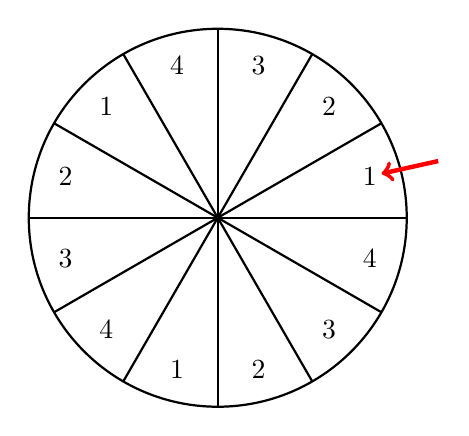
\begin{tikzpicture}[scale=.8]
        \foreach \i in {1,...,12} {
            \draw[thick] (0,0) -- ({30*\i}:3);
            %\node at ({30*(\i-0.5)}:2.5) {\i};
        }
        \foreach \i in {1,2,3,4} {
            \node at ({30*(\i-0.5)}:2.5) {\i};
            \node at ({30*(\i+3.5)}:2.5) {\i};
            \node at ({30*(\i+7.5)}:2.5) {\i};
        }
        \draw[thick] (0,0) circle(3);
        \draw[->, ultra thick, red] (3.5,.9) -- (2.6,.7); % Ajout de la flèche
    \end{tikzpicture}
}
\begin{enumerate}
    \item Quelle est la loi de probabilité suivie par $X$ ?
    \item Combien de points un joueur peut-il espérer gagner en moyenne lors d'une partie ?
    \item Pour pouvoir tourner la roue, le joueur doit payer 1 euro. Un point rapporte 0,40 €. Le jeu est-il équitable?
\end{enumerate}

\vspace*{.5cm}

\exo{}\\
En janvier 2025, la ville de Rennes a subit une crue exceptionnelle de l'Ille. La précédente crue semblable a eu lieu en 1981.\\
On suppose que les crues de l'Ille sont indépendantes entre elles, qu'il y a au plus une crue par an et que chaque année, une crue se réalise avec une probabilité égale à 0,02.

\subsection*{Période entre deux crues}
Soit $T$ la variable aléatoire égale au nombre d'années écoulées avant la prochaine crue de l'Ille.\\ 
\textit{Si nécessaire, on arrondira les résultats à $10^{-4}$ près.}
\begin{enumerate}
    \item Calculer $P(T=1)$ et interpréter le résultat.
    \item Calculer la probabilité que la prochaine crue de l'Ille se produise dans 10 ans.
    \item Quelle est la loi de probabilité suivie par $T$ ? Préciser son (ou ses) paramètre(s).
    \item Justifier qu'une telle crue se produit en moyenne tous les 50 ans.
\end{enumerate}

\subsection*{Nombre de crues par siècle}
Soit $N$ la variable aléatoire égale au nombre de crues de l'Ille pendant les 100 prochaines années.
\begin{enumerate}
    \item Quelle est la loi de probabilité suivie par $N$ ? Préciser son (ou ses) paramètre(s).
    \item Calculer la probabilité qu'il n'y ait pas de crue de l'Ille pendant les 100 prochaines années.
    \item En déduire la probabilité qu'il y ait au moins une crue de l'Ille pendant les 100 prochaines années.
    \item À l'aide de la calculatrice, déterminer la probabilité qu'il y ait au moins 5 crues de l'Ille pendant les 100 prochaines années.
\end{enumerate}

\vspace*{.5cm}

\exo{ Loi de refroidissement de Newton}\\
Une tasse de café est servie à une température initiale de 80°C. On la laisse refroidir dans une pièce à température ambiante de 20°C.\\
On va étudier à l'aide d'une suite le refroidissement du café en appliquant la loi de Newton.\\

Pour tout entier naturel $n$, on note $t_n$ la température du café (en °C)au bout de $n$ minutes.\\
On a ainsi $t_0=80$. Entre deux minutes consécutives $n$ et $n+1$, on a $t_{n+1}-t_n=-0,2(t_n-20)$.
\begin{enumerate}
    \item Conjecturer d'après le contexte le sens de variation de la suite $(t_n)$.
    \item Montrer que, pour tout entier naturel $n$, on a $t_{n+1}=0,8t_n+4$.
    \item Exprimer $t_n$ en fonction de $n$.
    \item Déterminer la limite de la suite $(t_n)$.
    \item \faCalculator \hspace*{.2cm} Combien de temps faut-il pour que la température du café soit inférieure à 30°C ?
\end{enumerate}
\end{document}